\documentclass{article}
\usepackage{tikz}
\usepackage{float}

\usepackage{caption}
\usepackage{subcaption}

\usetikzlibrary{automata,arrows,positioning,calc}
\usepackage{enumitem}
\usepackage{amssymb}
\usepackage{fontawesome}
\usepackage{pythonhighlight}
\usepackage{hyperref}

\renewcommand{\thesubsection}{\thesection.\alph{subsection}}
\newcommand{\quotes}[1]{``#1''}

\title{
    \textbf{Estruturas de Dados II}\\
    Grafos – Definições e Representações - V
}
\author{
    Augusto Emerson\\
    Felipe Monteiro\\
    Jaime Silva\\
    João Victor\\
    Nil Wakya Wai Wai\\
    Sandyella Soares 
}
\date{} % Remova a data

\begin{document}

\begin{titlepage}
    \maketitle
    \thispagestyle{empty}  
\end{titlepage}

\section{} % 1
    De acordo com Cormen, os dois tipos de grafos que existem são Grafos direcionados (ou digrafos) e Grafos não direcionados.
    
    Nos Grafos direcionados as arestas têm uma direção específica, indicando a relação de \quotes{origem} e \quotes{destino} entre os vértices. Em outras palavras, é possível percorrer as arestas em uma única direção. Já nos Grafos não direcionados as arestas não possuem direção, ou seja, não há uma relação de \quotes{origem} e \quotes{destino} entre os vértices. As arestas podem ser percorridas em ambas as direções.
    
    A principal diferença entre eles é a presença ou ausência de direção nas arestas, o que afeta a forma como a informação flui através do grafo.

\section{} % 2 
    \subsection{}
        % Dirigido
        % V = {1, 2, 3, 4, 5}
        % A = {(1, 2), (1, 4), (1, 5), (2, 3), (3, 4), (4, 4)}
        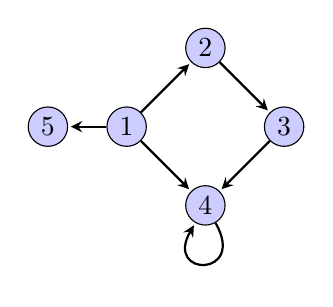
\begin{tikzpicture} [> = stealth,  shorten > = 1pt,   auto,   node distance = 1.5cm]
            % Estilo para os nós
            \tikzstyle{vertex}=[circle, draw, inner sep=0pt, minimum size=5mm]
            
            % Nós
            \node[vertex, fill=blue!20] (v1) at (-2,0) {1};
            \node[vertex, fill=blue!20] (v2) at (-1,1) {2};
            \node[vertex, fill=blue!20] (v3) at (0,0) {3};            
            \node[vertex, fill=blue!20] (v4) at (-1,-1) {4};
            \node[vertex, fill=blue!20] (v5) at (-3,0) {5};
            
            % Arestas
            \draw[->,thick] (v4) to [out=-60,in=-120,looseness=8] (v4);
            \draw[->,thick] (v1) -- (v2);
            \draw[->,thick] (v1) -- (v4);
            \draw[->,thick] (v1) -- (v5);
            \draw[->,thick] (v2) -- (v3);
            \draw[->,thick] (v3) -- (v4);
        \end{tikzpicture}
    \subsection{}
        % Dirigido: 
        % V = {1, 2, 3, 4}
        % A = {(1, 2), (2, 3), (2, 4), (3, 4), (4, 3), (3, 2)}
        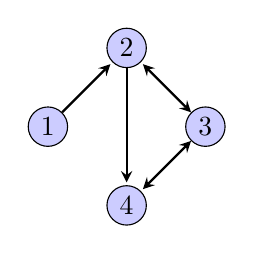
\begin{tikzpicture} [> = stealth,  shorten > = 1pt,   auto,   node distance = 1.5cm]
            % Estilo para os nós
            \tikzstyle{vertex}=[circle, draw, inner sep=0pt, minimum size=5mm]
            
            % Nós
            \node[vertex, fill=blue!20] (v1) at (-2,0) {1};
            \node[vertex, fill=blue!20] (v2) at (-1,1) {2};
            \node[vertex, fill=blue!20] (v3) at (0,0) {3};            
            \node[vertex, fill=blue!20] (v4) at (-1,-1) {4};
            
            % Arestas
            \draw[->,thick] (v1) -- (v2);
            \draw[->,thick] (v2) -- (v4);
            \draw[<->,thick] (v3) -- (v4);
            \draw[<->,thick] (v3) -- (v2);
        \end{tikzpicture}
    \subsection{}
        % Não Dirigido:
        % V = {1, 2, 3, 4, 5}
        % A = {(1, 2), (1, 4), (2, 3), (2, 4), (2, 5), (3, 4), (3, 5)}
        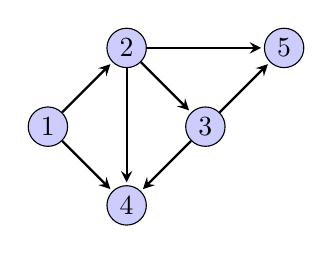
\begin{tikzpicture} [> = stealth,  shorten > = 1pt,   auto,   node distance = 1.5cm]
            % Estilo para os nós
            \tikzstyle{vertex}=[circle, draw, inner sep=0pt, minimum size=5mm]
            
            % Nós
            \node[vertex, fill=blue!20] (v1) at (-2,0) {1};
            \node[vertex, fill=blue!20] (v2) at (-1,1) {2};
            \node[vertex, fill=blue!20] (v3) at (0,0) {3};            
            \node[vertex, fill=blue!20] (v4) at (-1,-1) {4};
            \node[vertex, fill=blue!20] (v5) at (1,1) {5};
            
            % Arestas
            \draw[->,thick] (v1) -- (v2);
            \draw[->,thick] (v1) -- (v4);
            \draw[->,thick] (v2) -- (v3);
            \draw[->,thick] (v2) -- (v4);
            \draw[->,thick] (v2) -- (v5);
            \draw[->,thick] (v3) -- (v4);
            \draw[->,thick] (v3) -- (v5);
        \end{tikzpicture}     
    \subsection{}
        % Dirigido e não dirigido
        % V = {1, 2, 3, 4, 5, 6}
        % A = {(1, 2), (1, 3), (1, 4), (2, 5), (2, 6), (3, 5), (3, 6), (4, 5), (5, 6)}
        \begin{figure}[H]
            \begin{subfigure}{0.30\textwidth}
                \centering
                  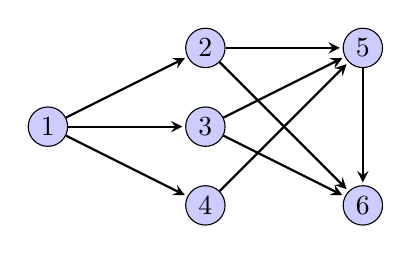
\begin{tikzpicture}[> = stealth,  shorten > = 1pt,   auto,   node distance = 1.5cm]
                       \tikzstyle{vertex}=[circle, draw, inner sep=0pt, minimum size=5mm]
            
                        % Nós
                        \node[vertex, fill=blue!20] (v1) at (-3,0) {1};
                        \node[vertex, fill=blue!20] (v2) at (-1,1) {2};
                        \node[vertex, fill=blue!20] (v3) at (-1,0) {3};            
                        \node[vertex, fill=blue!20] (v4) at (-1,-1) {4};
                        \node[vertex, fill=blue!20] (v5) at (1,1) {5};
                        \node[vertex, fill=blue!20] (v6) at (1,-1) {6};
                        
                        % Arestas
                        \draw[->,thick] (v1) -- (v2);
                        \draw[->,thick] (v1) -- (v3);
                        \draw[->,thick] (v1) -- (v4);
                        \draw[->,thick] (v2) -- (v5);
                        \draw[->,thick] (v2) -- (v6);
                        \draw[->,thick] (v3) -- (v5);
                        \draw[->,thick] (v3) -- (v6);
                        \draw[->,thick] (v4) -- (v5);
                        \draw[->,thick] (v5) -- (v6);
                  \end{tikzpicture}
                \caption{Dirigido}
            \end{subfigure}
            \hspace{1.5cm}
            \begin{subfigure}{\textwidth}
                \centering
                  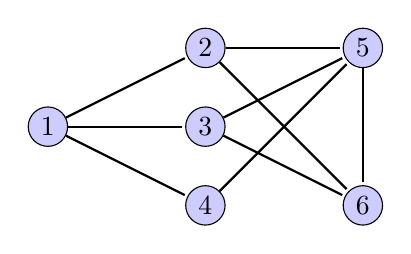
\begin{tikzpicture}[> = stealth,  shorten > = 1pt,   auto,   node distance = 1.5cm]
                       \tikzstyle{vertex}=[circle, draw, inner sep=0pt, minimum size=5mm]
            
                        % Nós
                        \node[vertex, fill=blue!20] (v1) at (-3,0) {1};
                        \node[vertex, fill=blue!20] (v2) at (-1,1) {2};
                        \node[vertex, fill=blue!20] (v3) at (-1,0) {3};            
                        \node[vertex, fill=blue!20] (v4) at (-1,-1) {4};
                        \node[vertex, fill=blue!20] (v5) at (1,1) {5};
                        \node[vertex, fill=blue!20] (v6) at (1,-1) {6};
                        
                        % Arestas
                        \draw[-,thick] (v1) -- (v2);
                        \draw[-,thick] (v1) -- (v3);
                        \draw[-,thick] (v1) -- (v4);
                        \draw[-,thick] (v2) -- (v5);
                        \draw[-,thick] (v2) -- (v6);
                        \draw[-,thick] (v3) -- (v5);
                        \draw[-,thick] (v3) -- (v6);
                        \draw[-,thick] (v4) -- (v5);
                        \draw[-,thick] (v5) -- (v6);
                  \end{tikzpicture}
                \caption{Não Dirigido}
          \end{subfigure}
        \end{figure}
\section{} % 3
    \subsection{}
        \begin{figure}[H]
            \begin{minipage}{0.8\textwidth}
                \centering
                \captionsetup{labelformat=empty}
                \caption{Listas de Adjacência}
            \end{minipage}
            \centering
            \begin{subfigure}{0.30\textwidth}
                \begin{tabular}{l | l}
                    \Large 1 & \Large $\rightarrow$ 2 $\rightarrow$ 3 $\rightarrow$ 5\\
                    \Large 2 & \Large $\rightarrow$ 3\\
                    \Large 3 & \Large $\rightarrow$ 4\\
                    \Large 4 & \Large $\rightarrow$ 4\\
                    \Large 5 & \\
                \end{tabular}
            \end{subfigure}
        \end{figure}
        \begin{figure}[H]
            \begin{minipage}{0.8\textwidth}
                \centering
                \captionsetup{labelformat=empty}
                \caption{Matriz de Adjacência}
            \end{minipage}
            \centering
            \begin{subfigure}{0.30\textwidth}
                \begin{tabular}{c|ccccc}
                      & 1 & 2 & 3 & 4 & 5 \\
                \hline
                    1 & 0 & 1 & 0 & 1 & 1 \\
                    2 & 0 & 0 & 1 & 0 & 0 \\
                    3 & 0 & 0 & 0 & 1 & 0 \\
                    4 & 0 & 0 & 0 & 1 & 0 \\
                    5 & 0 & 0 & 0 & 0 & 0 \\
                \end{tabular}
            \end{subfigure}
        \end{figure}
    \subsection{}
        \begin{figure}[H]
            \begin{minipage}{0.8\textwidth}
                \centering
                \captionsetup{labelformat=empty}
                \caption{Listas de Adjacência}
            \end{minipage}
            \centering
            \begin{subfigure}{0.30\textwidth}
                \begin{tabular}{l | l}
                    \Large 1 & \Large $\rightarrow$ 2\\
                    \Large 2 & \Large $\rightarrow$ 3 $\rightarrow$ 4\\
                    \Large 3 & \Large $\rightarrow$ 4 $\rightarrow$ 2\\
                    \Large 4 & \Large $\rightarrow$ 3\\
                \end{tabular}
            \end{subfigure}
        \end{figure}
        \begin{figure}[H]
            \begin{minipage}{0.8\textwidth}
                \centering
                \captionsetup{labelformat=empty}
                \caption{Matriz de Adjacência}
            \end{minipage}
            \centering
            \begin{subfigure}{0.30\textwidth}
                \begin{tabular}{c|cccc}
                      & 1 & 2 & 3 & 4 \\
                \hline
                    1 & 0 & 1 & 0 & 0 \\
                    2 & 0 & 0 & 1 & 1 \\
                    3 & 0 & 1 & 0 & 1 \\
                    4 & 0 & 0 & 1 & 0 \\
                \end{tabular}
            \end{subfigure}
        \end{figure}
    \subsection{}
        \begin{figure}[H]
            \begin{minipage}{0.8\textwidth}
                \centering
                \captionsetup{labelformat=empty}
                \caption{Listas de Adjacência}
            \end{minipage}
            \centering
            \begin{subfigure}{0.30\textwidth}
                \begin{tabular}{l | l}
                    \Large 1 & \Large $\rightarrow$ 2 $\rightarrow$ 4\\
                    \Large 2 & \Large $\rightarrow$ 3 $\rightarrow$ 4 $\rightarrow$ 5\\
                    \Large 3 & \Large $\rightarrow$ 4 $\rightarrow$ 5\\
                    \Large 4 & \Large\\
                    \Large 5 & \Large\\
                \end{tabular}
            \end{subfigure}
        \end{figure}
        \begin{figure}[H]
            \begin{minipage}{0.8\textwidth}
                \centering
                \captionsetup{labelformat=empty}
                \caption{Matriz de Adjacência}
            \end{minipage}
            \centering
            \begin{subfigure}{0.30\textwidth}
                \begin{tabular}{c|ccccc}
                      & 1 & 2 & 3 & 4 & 5 \\
                \hline
                    1 & 0 & 1 & 0 & 1 & 0 \\
                    2 & 1 & 0 & 1 & 1 & 1 \\
                    3 & 0 & 1 & 0 & 1 & 1 \\
                    4 & 1 & 1 & 1 & 0 & 0 \\
                    5 & 0 & 1 & 1 & 0 & 0 \\
                \end{tabular}
            \end{subfigure}
        \end{figure}    
    \subsection{}
        \begin{figure}[H]
            \begin{minipage}{0.8\textwidth}
                \centering
                \captionsetup{labelformat=empty}
                \caption{Listas de Adjacência}
            \end{minipage}
            \centering
            \begin{subfigure}{0.30\textwidth}
                \begin{tabular}{l | l}
                    \Large 1 & \Large $\rightarrow$ 2 $\rightarrow$ 3 $\rightarrow$ 4\\
                    \Large 2 & \Large $\rightarrow$ 5 $\rightarrow$ 6\\
                    \Large 3 & \Large $\rightarrow$ 5 $\rightarrow$ 6\\
                    \Large 4 & \Large $\rightarrow$ 5\\
                    \Large 5 & \Large $\rightarrow$ 6\\
                    \Large 6 & \Large\\
                \end{tabular}
                \caption{Dirigido}
            \end{subfigure}
            \hspace{1.5cm}
            \centering
            \begin{subfigure}{0.30\textwidth}
                \begin{tabular}{l | l}
                    \Large 1 & \Large $\rightarrow$ 2 $\rightarrow$ 3 $\rightarrow$ 4\\
                    \Large 2 & \Large $\rightarrow$ 1 $\rightarrow$ 5 $\rightarrow$ 6\\
                    \Large 3 & \Large $\rightarrow$ 1 $\rightarrow$ 5 $\rightarrow$ 6\\
                    \Large 4 & \Large $\rightarrow$ 1 $\rightarrow$ 5\\
                    \Large 5 & \Large $\rightarrow$ 4 $\rightarrow$ 2 $\rightarrow$ 3 $\rightarrow$ 6\\
                    \Large 6 & \Large $\rightarrow$ 5 $\rightarrow$ 2 $\rightarrow$ 3\\
                \end{tabular}
                \caption{Não Dirigido}
            \end{subfigure}
        \end{figure}
        \begin{figure}[H]
            \begin{minipage}{0.8\textwidth}
                \centering
                \captionsetup{labelformat=empty}
                \caption{Matrizes de Adjacência}
            \end{minipage}
            \centering
            \begin{subfigure}{0.30\textwidth}
                \[
                    \begin{array}{c|cccccc}
                          & 1 & 2 & 3 & 4 & 5 & 6 \\
                    \hline
                        1 & 0 & 1 & 1 & 1 & 0 & 0 \\
                        2 & 0 & 0 & 0 & 0 & 1 & 1 \\
                        3 & 0 & 0 & 0 & 0 & 1 & 1 \\
                        4 & 0 & 0 & 0 & 0 & 1 & 0 \\
                        5 & 0 & 0 & 0 & 0 & 0 & 1 \\
                        6 & 0 & 0 & 0 & 0 & 0 & 0 \\
                    \end{array}
                \]
                \caption{Dirigido}
            \end{subfigure}
            \hspace{1.5cm}
            \centering
            \begin{subfigure}{0.30\textwidth}
                \[
                    \begin{array}{c|cccccc}
                          & 1 & 2 & 3 & 4 & 5 & 6 \\
                    \hline
                        1 & 0 & 1 & 1 & 1 & 0 & 0 \\
                        2 & 1 & 0 & 0 & 0 & 1 & 1 \\
                        3 & 1 & 0 & 0 & 0 & 1 & 1 \\
                        4 & 1 & 0 & 0 & 0 & 1 & 0 \\
                        5 & 0 & 1 & 1 & 1 & 0 & 1 \\
                        6 & 0 & 1 & 1 & 0 & 1 & 0 \\
                    \end{array}
                \]
                \caption{Não Dirigido}
            \end{subfigure}
        \end{figure}

\section{} % 4
    Um gráfico é considerado \quotes{esparso} quando o número de arestas é significavamente menor do que o número máximo de arestas que poderiam existir em um gráfico com o mesmo número de vértices. Por outro lado, um gráfico é considerado \quotes{denso} quando o número de arestas se aproxima ou é próximo do número máximo de arestas que poderiam existir. 
    
    A densidade de um grafo é geralmente expressa em termos de uma proporção (número de arestas / número máximo de arestas).
\section{} % 5
     A principal vantagem da matriz de adjacência sobre a lista de adjacência é a eficiência na verificação da presença de uma aresta específica entre dois vértices. Isso ocorre porque em uma matriz de adjacência, essa verificação é feita em tempo constante ($O(1)$), independentemente do tamanho do grafo.
\section{} % 6
    \subsection{}
        \begin{itemize}
            \item[] (\textcolor{red}{F}) É um grafo dirigido
            \item[] (\textcolor{green}{V}) É um grafo acíclico
            \item[] (\textcolor{green}{V}) Pode ser ponderado
            \item[] (\textcolor{green}{V}) O vértice 1 é acessível a partir do vértice 0
            \item[] (\textcolor{green}{V}) É um grafo conexo
            \item[] (\textcolor{red}{F}) É um grafo completo
        \end{itemize}
    \subsection{}
        \begin{itemize}
            \item[] (\textcolor{green}{V}) É um grafo dirigido
            \item[] (\textcolor{green}{V}) É um grafo acíclico
            \item[] (\textcolor{green}{V}) É um grafo fortemente conexo
            \item[] (\textcolor{green}{V}) O vértice 8 é adjacente do 3
            \item[] (\textcolor{red}{F}) O vértice 5 é adjacente do 11
            \item[] (\textcolor{green}{V}) O grau de maior valor é 3
            \item[] (\textcolor{green}{V}) Existe um caminho 〈9, 11, 5〉
            \item[] (\textcolor{red}{F}) Existe um caminho 〈3, 8, 9〉
            \item[] (\textcolor{red}{F}) Pode ser organizado como um grafo bipartido
        \end{itemize}
\section{} % 7
\begin{python}
class Vertex:
    def __init__(self, index, name=None, data=None):
        self.index = index
        self.name = name
        self.data = data
    
\end{python}
\href{https://github.com/aejunior/bsi-ed-ii/blob/master/src/graph/Vertex.py}{\faGithub}

\section{} % 8
\begin{python}
class Edge:
    def __init__(self, source, target, is_directed=True, weight=None, data=None):
        self.source = source
        self.target = target
        self.is_directed = is_directed
        self.weight = weight
        self.data = data
\end{python}
\href{https://github.com/aejunior/bsi-ed-ii/blob/master/src/graph/Edge.py}{\faGithub}

\section{} % 9
\begin{python}
from .Graph import Graph
from .Vertex import Vertex
from .Edge import Edge



class AdjacencyListGraph(Graph):
    def __init__(self):
        self.graph = {}
        self.num_vertices = 0

    def numberOfVertices(self):
        return self.num_vertices

    def numberOfEdges(self):
        count = 0
        for vertex in self.graph:
            count += len(self.graph[vertex])
        return count

    def addVertex(self, name: str = None, data: object = None):
        if name is None:
            name = self.num_vertices
        self.graph[name] = []
        self.num_vertices += 1
        return Vertex(name, name, data)

    def vertexAt(self, i: int):
        vertices = list(self.graph.keys())
        if i < len(vertices):
            return Vertex(vertices[i], vertices[i], self.graph[vertices[i]])

    def addEdge(self, ui: int, vi: int, isDirected: bool = True, weight=None, data=None):
        if ui not in self.graph:
            self.addVertex(ui)
        if vi not in self.graph:
            self.addVertex(vi)
        edge = Edge(ui, vi, isDirected, weight, data)
        self.graph[ui].append(edge)
        if not isDirected:
            reverse_edge = Edge(vi, ui, isDirected, weight, data)
            self.graph[vi].append(reverse_edge)
        return edge

    def edgeExists(self, ui: int, vi: int):
        if ui in self.graph:
            for edge in self.graph[ui]:
                if edge.target == vi:
                    return True
        return False

    def vertices(self):
        return [Vertex(name, name, self.graph[name]) for name in self.graph.keys()]

    def edges(self):
        all_edges = []
        for vertex in self.graph:
            for edge in self.graph[vertex]:
                all_edges.append(edge)
        return all_edges

    def outgoingEdgesFromVertex(self, ui: int):
        if ui in self.graph:
            return self.graph[ui]

    def adjacentVertices(self, ui: int):
        if ui in self.graph:
            adjacent_vertices = []
            for edge in self.graph[ui]:
                adjacent_vertices.append(edge.target)
            return adjacent_vertices
\end{python}
\href{https://github.com/aejunior/bsi-ed-ii/blob/master/src/graph/alg.py}{\faGithub}

\section{} % 10
\begin{python}
from .Graph import Graph
from .Vertex import Vertex
from .Edge import Edge



class AdjacencyMatrixGraph(Graph):
    def __init__(self):
        self.graph = {}
        self.num_vertices = 0
        self.matrix = []

    def numberOfVertices(self):
        return self.num_vertices

    def numberOfEdges(self):
        count = 0
        for row in self.matrix:
            count += sum(row)
        return count

    def addVertex(self, name: str = None, data: object = None):
        if name is None:
            name = self.num_vertices
        self.graph[name] = data
        self.num_vertices += 1
        for row in self.matrix:
            row.append(0)
        self.matrix.append([0] * self.num_vertices)
        return Vertex(name, name, data)

    def vertexAt(self, i: int):
        vertices = list(self.graph.keys())
        if i < len(vertices):
            return Vertex(vertices[i], vertices[i], self.graph[vertices[i]])

    def addEdge(self, ui: int, vi: int, isDirected: bool = True, weight=None, data=None):
        if ui >= self.num_vertices or vi >= self.num_vertices:
            raise ValueError("Vertex not found")
        self.matrix[ui][vi] = 1
        if not isDirected:
            self.matrix[vi][ui] = 1
        return Edge(ui, vi, isDirected, weight, data)

    def edgeExists(self, ui: int, vi: int):
        if ui >= self.num_vertices or vi >= self.num_vertices:
            return False
        return self.matrix[ui][vi] == 1

    def vertices(self):
        return [Vertex(name, name, self.graph[name]) for name in self.graph.keys()]

    def edges(self):
        edges = []
        for i in range(self.num_vertices):
            for j in range(self.num_vertices):
                if self.matrix[i][j] == 1:
                    edges.append(Edge(i, j, True, None, None))
        return edges

    def outgoingEdgesFromVertex(self, ui: int):
        edges = []
        for i in range(self.num_vertices):
            if self.matrix[ui][i] == 1:
                edges.append(Edge(ui, i, True, None, None))
        return edges

    def adjacentVertices(self, ui: int):
        adjacent_vertices = []
        for i in range(self.num_vertices):
            if self.matrix[ui][i] == 1:
                adjacent_vertices.append(i)
        return adjacent_vertices
\end{python}
\href{https://github.com/aejunior/bsi-ed-ii/blob/master/src/graph/amg.py}{\faGithub}

\end{document}